\documentclass[../../../OAE-SPEC-MAIN.tex]{subfiles}
\begin{document}

%\title{From Ethernet to Chiplet Æthernet}

%\subsection{Æthernet Design Philosophy}
\section{From Ethernet to Æthernet}

%\begin{marginfigure}
%  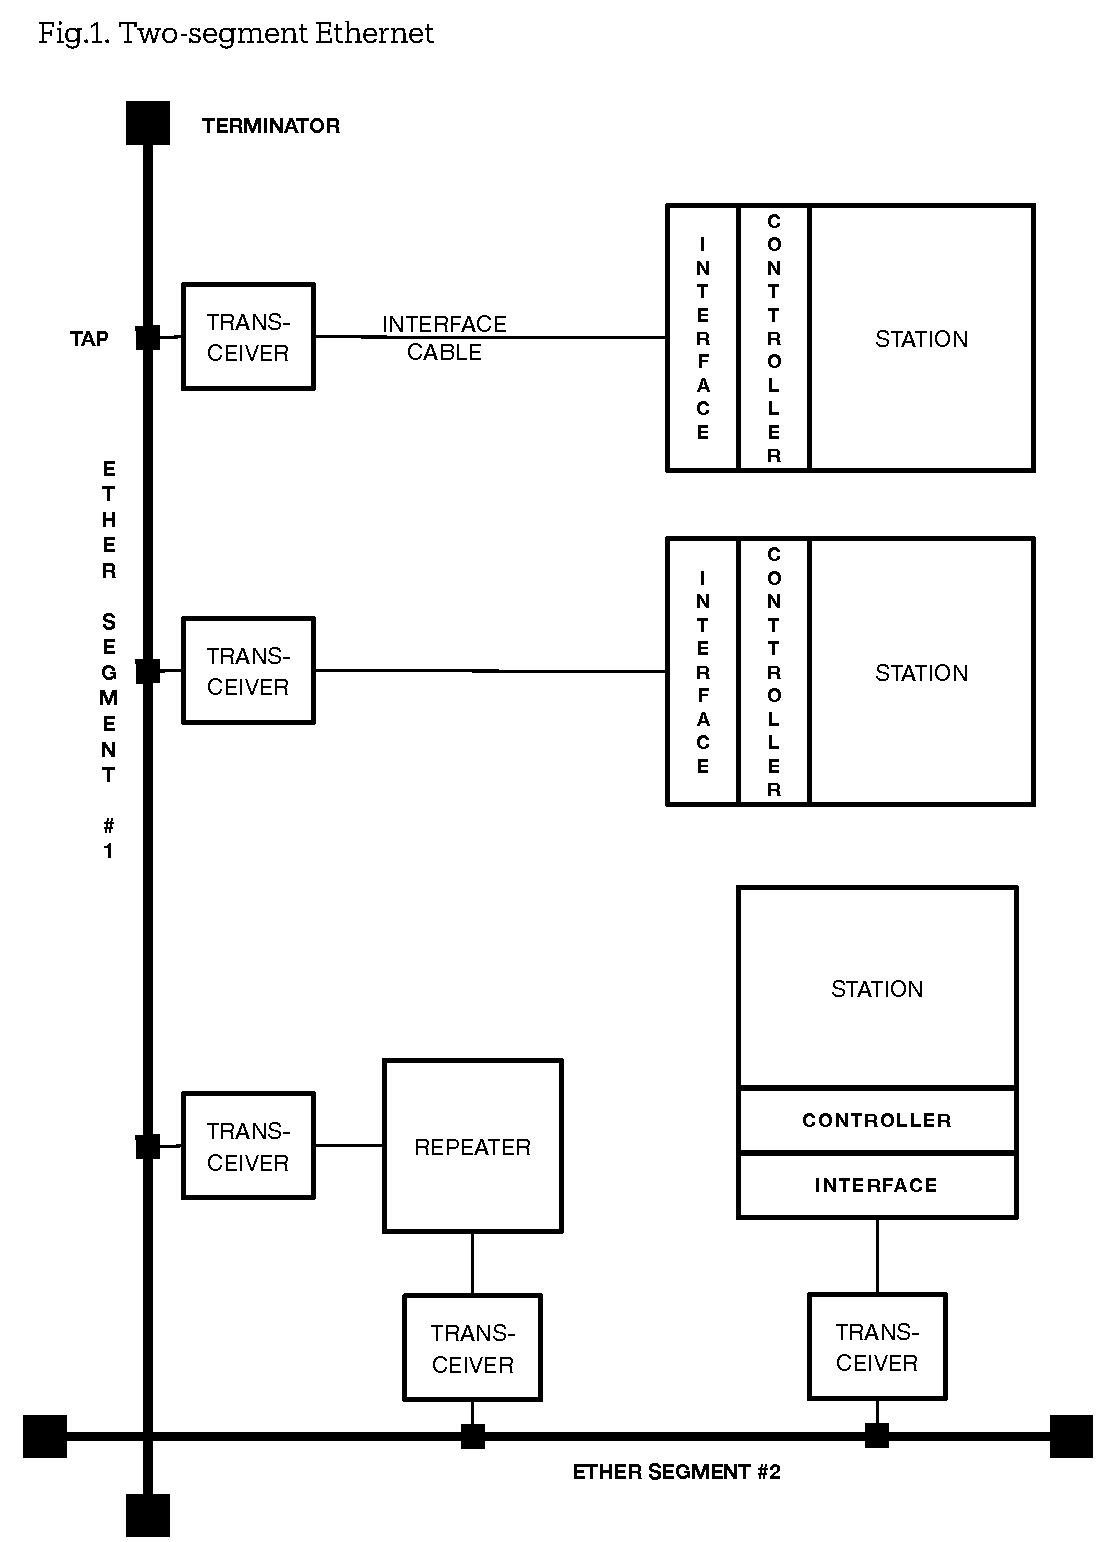
\includegraphics[width=1.2\linewidth]{../../FIGURES/Omni-Figure-1.pdf}
%  \caption{Original Ethernet Concepts} %& Terminology}
%  \vspace{2em}
%\end{marginfigure}

\marginfig[width=1.2\linewidth, trim=0mm 0mm 0mm 18mm, clip]{Omni-Figure-1.pdf}[Original Ethernet Concepts]
It would be a mistake to assume conventional network concepts and terminology that you already know and love will remain unscathed in this project. While we have no intention of reinventing the wheel,  some new concepts and terminology will be necessary in order to escape the quagmire of incrementalism of the last five decades.  

%\marginnote{We carefully described in four presentations why the concept of time is widely misunderstood in the OCP TAP (Time Appliance Community).  We respectfully request that you watch those presentations before insisting on timestamps or synchronized time in the context of Open Atomic Ethernet. \href{https://www.opencompute.org/w/index.php?title=Open_Atomic_Ethernet}{Open Atomic Ethernet}}

 
\marginfig[width=1.2\linewidth]{Original-Ethernt.pdf}[Ethernet Components]
%\section{From Ethernet to AEthernet}

\subsection{Ethernet was Born}

The Original concepts of Ethernet, developed 50 years ago, help us understand the thinking, theoretical concepts, and guide us  to practical implementations. It is important to understand the design philosophy, so we can learn the most from the intuition that created the Ethernet revolution.  It is instructive to trace the initial intellectual and conceptual steps when Ethernet was first developed, and make sure we are not missing some invaluable intuition.


  
\marginfig[width=1.2\linewidth]{Bipartite.pdf}[Chiplet Æthernet: HDX/FDX]
   
The original Ethernet was a single coax cable (photon cavity) Half-Duplex `Bus':  alternating between listening and transmitting in `slots' on the bus.
\bigskip
 
These temporal `slots' were time \emph{intervals}: controlled and measured against a local oscillator (often a crystal), which had their own drift and stability characteristics. In a half-duplex world, such as on a single coax cable, this meant that the Transceiver (Transmitter + Receiver) would transmit for half the `time' and listen for the other half the `time', and be able to detect collisions (the receiver monitors what it itself is transmitting and compares it to what it is receiving to see. 

The transmitting station is immediately provided with electrical (signal) feedback which lets it see (a) that it's transmitter  was working, and (b) what other receivers might be seeing. From a Shannon perspective, we call this \emph{Initial Information-Feedback (IIF)} and reserve the definition of \emph{Perfect Information Feedback (PIF} for the case where the SerDes at the other end is reflecting what it sees.  See section XX for the full theory behind the Dual Back-to-Back (DB2B) Shannon model works.

\subsection{Ethernet Evolves}

Ethernet rapidly evolved to a full duplex situation where there are two separate connections to the media.  One in the transmit direction, and one in the receive direction. However, if one direction is working, and the other direction is not, we could always (in Æthernet) revert back to communicating independently on each cable.  This may not have the ideal performance characteristics, but remains a valuable redundancy tool to locally diagnose (and report) unidirectional errors, and flakey fiber connections. This is effectively a dual redundant `communication' verification tool that can be algorithmically self diagnosing, perhaps in combination to Link training in Modern Ethernet. 

\section{AEthernet Configuration}

\marginfig{Chiplet-XPU.pdf}[Uninitialized XPU Links]


We begin with two cells, and extend to three. This is the minimum irreducible graph for healing around a broken link. Links can be broken in both directions, or one direction at a time (unidirectional failures) 

\section{Chiplet XPUs}
\section{Configured Links}
\marginfig{Configured-Links.pdf}[Configured Links for TX/RX]



We go from Chiplet Servers to something more generalized - XPU's 


This $3 \times 3$ Tile is the basic fault-tolerant Tile.


Unactivated Links go from being dead to being alive by exchanging configuration packets. These establish the \emph{direction} of the links from 

 
\marginfig[width=1.2\linewidth]{3x3-wire-hop-chiplets}
 
 \section{From Repeaters to Switches to Routers, and Back to Repeaters}
 
 Bob Metcalfe's concept of a repeater was like what Heaviside discovered -- a device to take a fading signal and boost it to recreate a strong signal so as to propagate further. That was the simplistic `engineers' view of how it worked.  The `physicist's view' was far more interesting -- they took a transmission line model, where characteristic impedance $Z_o = \sqrt{{\frac{L_o}{C_o}}}$. %For a lossless Transmission line, this number is real.
 
 It would be a mistake to assume conventional network concepts and terminology that you already know and love will remain unscathed in this project. While we have no intention of reinventing the wheel,  some new concepts and terminology will be necessary in order to escape the quagmire of incrementalism of the last five decades.  


 \section{Minimum Triangle}
 
\marginfig[width=1.2\linewidth]{Minimum-Triangle.pdf}

LOREM IPSUM It would be a mistake to assume conventional network concepts and terminology that you already know and love will remain unscathed in this project. While we have no intention of reinventing the wheel,  some new concepts and terminology will be necessary in order to escape the quagmire of incrementalism of the last five decades.  

\marginfig[width=1.2\linewidth]{8x10-Chiplets.pdf}


\section{Big Flexible Chiplet}

LOREM IPSUM It would be a mistake to assume conventional network concepts and terminology that you already know and love will remain unscathed in this project. While we have no intention of reinventing the wheel,  some new concepts and terminology will be necessary in order to escape the quagmire of incrementalism of the last five decades.  


\marginfig[width=1.2\linewidth]{Big-Flexible-Chipet.pdf}


\section{Links are primary communication resources}

The link between Alice and Bob is the resource to be shared.  What goes over this link is controlled entirely by Alice and Bob.

The GAME the protocol plays ensures \emph{fairness} (50/50 sharing of the link resources). Whatever is left over is offered as a resource to other cells further away.

This removes the need for POLICY -- Each link has it's own policy, and can use as much of the bandwidth they need to perform their computation.

Whatever is left over can be offered (advertised) to the rest of the system as a utilization path.

\clearpage

\fig[width=1.6\linewidth]{One-Link.pdf}[How routing Works]

\clearpage

\section{Colored Big Picture}
\fig[width=1.6\linewidth]{Chiplet-Colors.pdf}[From indistinguishable XPU's to self-distinguished Roots of the Scouting Tree]

\clearpage


\section{From Physical Cells (XPUs) to Logical Tiles}

\section{Consensus Tiles} 1

\marginfig{ConsensusTile.pdf}[Consensus Tiles]

\section{Logical Tiles}

Logical Tiles are built on top of physical tiles.  They have the same 3x3 failure independence characteristics, but help define failure boundaries (the shared fate) of the system. These are discovered, not configured.  

Because these 


\marginfig{tensor-Tile-8x8.pdf}[3 x 3 tile]

\section{Tiles -2}

\marginfig{tensor-tile-9x9.pdf}[9 x 9 Logical Mesh]

\section{Consensus Tiles 3}

LOREM IPSUM It would be a mistake to assume conventional network concepts and terminology that you already know and love will remain unscathed in this project. While we have no intention of reinventing the wheel,  some new concepts and terminology will be necessary in order to escape the quagmire of incrementalism of the last five decades.  

\marginfig{tensor-tile-12x12.pdf}[9 x 9 Logical Mesh]

LOREM IPSUM It would be a mistake to assume conventional network concepts and terminology that you already know and love will remain unscathed in this project. While we have no intention of reinventing the wheel,  some new concepts and terminology will be necessary in order to escape the quagmire of incrementalism of the last five decades.  

\section{Logical Overlays}\

LOREM IPSUM It would be a mistake to assume conventional network concepts and terminology that you already know and love will remain unscathed in this project. While we have no intention of reinventing the wheel,  some new concepts and terminology will be necessary in order to escape the quagmire of incrementalism of the last five decades.  

\subsection{Unfolded Clos}

LOREM IPSUM It would be a mistake to assume conventional network concepts and terminology that you already know and love will remain unscathed in this project. While we have no intention of reinventing the wheel,  some new concepts and terminology will be necessary in order to escape the quagmire of incrementalism of the last five decades.  

\marginfig[width=1.2\linewidth]{Unfolded-Clos.pdf}[Unfolded Clos]

\subsection{Virtual Unfolded Clos}

LOREM IPSUM It would be a mistake to assume conventional network concepts and terminology that you already know and love will remain unscathed in this project. While we have no intention of reinventing the wheel,  some new concepts and terminology will be necessary in order to escape the quagmire of incrementalism of the last five decades.  

\marginfig[width=1.2\linewidth]{Virtual-Unfolded-Clos.pdf}[Virtual Unfolded Clos. Fish-Eye View of the LINK from any arbitrary LINK]


\section{Physical Overlays}

LOREM IPSUM It would be a mistake to assume conventional network concepts and terminology that you already know and love will remain unscathed in this project. While we have no intention of reinventing the wheel,  some new concepts and terminology will be necessary in order to escape the quagmire of incrementalism of the last five decades.  

\section{Dragonfly}

LOREM IPSUM It would be a mistake to assume conventional network concepts and terminology that you already know and love will remain unscathed in this project. While we have no intention of reinventing the wheel,  some new concepts and terminology will be necessary in order to escape the quagmire of incrementalism of the last five decades.  

\marginfig[width=1.2\linewidth]{HexTensor.pdf}[Fish-Eye Lens View of the network from an arbitrary Cell]
      \vspace{2em}

\end{document}
